\chapter{Submanifolds}
\section{Basic definitions}

\begin{definition*}
    Let \(M\) be a topological manifolds. A subset \(S\subset M\) is a \dhighlight{topological submanifold},
    if \(S\) is a topological manifold with the subspace topology.
\end{definition*}

\begin{example}
    \(S^n=\{(x_0,\dots,x_n)\mid \sum x_i^2=1\}\subset\R^{1+n}\)
\end{example}
\begin{example}[Non-example]
    \(\{(x,y)\mid x=0\lor y=0\}\subset\R^2\), since this is not a manifold (see sheet 01).
\end{example}
\begin{definition*}
    Let \(M\) be a smooth manifold. A topological submanifold \(S\subset M\) is a \dhighlight{smooth submanifold}, if 
    it is equipped with a smooth structure, s.t. the embedding \(i:S\hookrightarrow M\) is smooth.   
\end{definition*}

\begin{example}
    If \(M\) is a smooth manifold and \(U\subset M\) open, then \(U\subset M\) is a smooth manifold.\marginnote{With the restricted smooth structure of \(M\)}
\end{example}

%examples should not be inside tcolorboxes?

\begin{remark}
    Some authors (including Lee's textbook) use the term \dhighlight{embedded submanifold} to distinguish 
    from \dhighlight{immersed submanifolds}. For use ``submanifolds''\(\equiv\)``embedded submanifold''.
\end{remark}  

\begin{lemma}\label{lem:5.1}
    Suppose that \(f:M\to N\) smooth embedding. Let \(S\coloneqq F(M)\subset N\). Then 
    \(S\) admits a unique smooth structure making it a smooth submanifold, with the property that 
    \(f\) is a diffeomorphism onto its image.
\end{lemma}

\begin{proof}
    By definition of \(f\) being an embedding, \(f\) is a homeomorphism onto it's image, with the subspace topology.
    \(\implies S\) is a topological manifold. 

    We define a smooth atlas on \(S\) by taking \(\{(f(U),\varphi\circ f^{-1})\}\), as \((U,\varphi)\) ranges over the set of charts 
    for \(M\).

    Clearly \(f\) is a diffeomorphism, since \(\varphi\circ f\circ f^{-1}\circ\psi^{-1}\), for \((U,\varphi),(V,\psi)\) smooth charts, this follows 
    from the fact that \((U,\varphi),(V,\psi)\) are smoothly compatible on \(M\).

    This is the only smooth at with the property that \(f\) is a diffeomorphism, if \(\cB\) is an other such atlas, then the fact 
    that \(f\) is a diffeomorphism for \((S,\cB)\iff (S,\cA)\) compatible.

    Finally
    \begin{figure}[H]
        \centering
        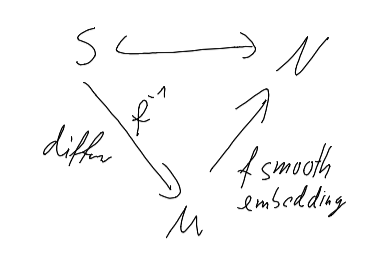
\includegraphics[width=.7\textwidth]{sketch_5_01.png}
        \caption{Sketch 5.01}
    \end{figure}
    so \(i\) is a smooth embedding.
\end{proof} 

\begin{definition*}
    A embedded submanifold \(S\) is called \dhighlight{properly embedded}, if the inclusion map 
    \(i\hookrightarrow N\) is proper (i.e. the preimage of a compact set is compact). 
\end{definition*}

\begin{example}
    \(S^n\hookrightarrow R^{n+1}\) properly embedded. 
\end{example}

\begin{example}[Non-example]
    \(S^n\setminus\{\text{pt}\}\subset\R^{n+1}\)
    \begin{figure}[H]
        \centering
        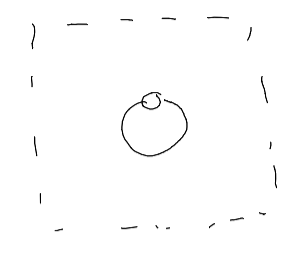
\includegraphics[width=.7\textwidth]{sketch_5_02.png}
        \caption{Sketch 5.02}
    \end{figure}
\end{example}

\begin{lemma}\label{lem:5.2}
    A topological submanifold \(S\subset N\) is properly embedded iff 
    \(S\) is closed.
\end{lemma}

\begin{proof}
    Exercise.\marginnote{Elementary exercise in point set topology}
\end{proof}

\section{The ``slice lemma''}

\begin{theorem}[Slice theorem]\label{thm:5.3}
    \begin{enumerate}
        \item[(a)] Suppose \(S^k\subset M^n\) is a Submanifold of codimension \(n-k\).\marginnote{this is also a definition of codimension: \(\dim M - \dim S\)}
                   Then, for all \(p\in S\), there exists a chart \((U,\varphi),p\in U\subset M\), such that \[\varphi(U\cap S)=\{(x_1,\dots,x_k,x_{k+1},\dots,x_n)\in \varphi(U)\mid x_{k+1}=c_{k+1},\dots,x_{n}=c_n\}.\]  
        \begin{figure}[H]
            \centering
            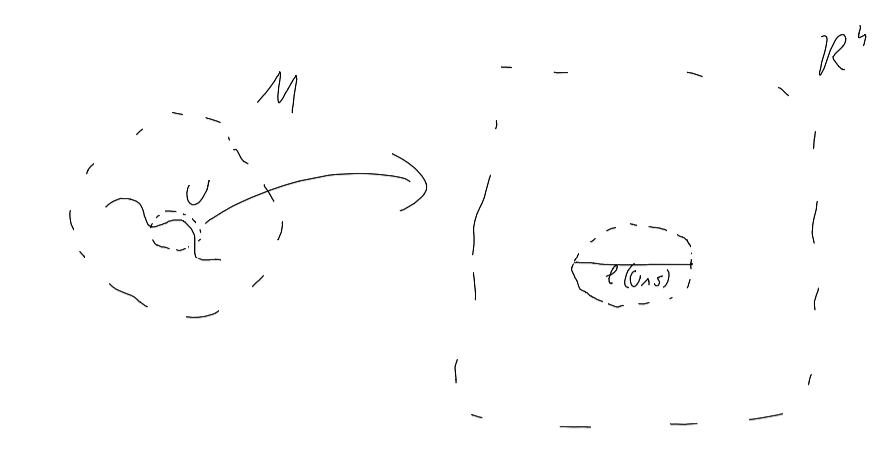
\includegraphics[width=.7\textwidth]{sketch_5_03.png}
            \caption{Sketch 5.03} 
        \end{figure}\markeol{09}
        \item[(b)] Done next time
    \end{enumerate}
\end{theorem}

